%\newpage
\section{Model pojazdu}
Na potrzeby symulacji utworzony został odpowiedni model samochodu. W tym celu wykorzystane zostały możliwości edycji obiektów dostępne w programie V-REP. Jako baza posłużył jeden z modeli, obecny w oprogramowaniu po jego instalacji, o nazwie 'simple Ackermann steering.ttm'. Model ten wyposażony był w funkcjonalne koła przymocowane do podstawy oraz podstawowe oprogramowanie umożliwiające sterowanie pojazdem z wykorzystaniem klawiatury.

W celu przystosowania modelu do naszych potrzeb wykonany został szereg akcji. Model upodobniono wyglądem do realnego pojazdu poprzez dodanie dodatkowych kształtów, co z pewnością pozytywnie wpłynie na wizualny odbiór symulacji. Dodane zostały między innymi atrapy takich elementów jak szyby, opony oraz reflektory. Z modelu zostały także usunięte zbędne elementy, takie jak linie pokazujące skręcenie osi poszczególnych kół podczas symulacji.

\begin{figure}[!h]
	\centering
	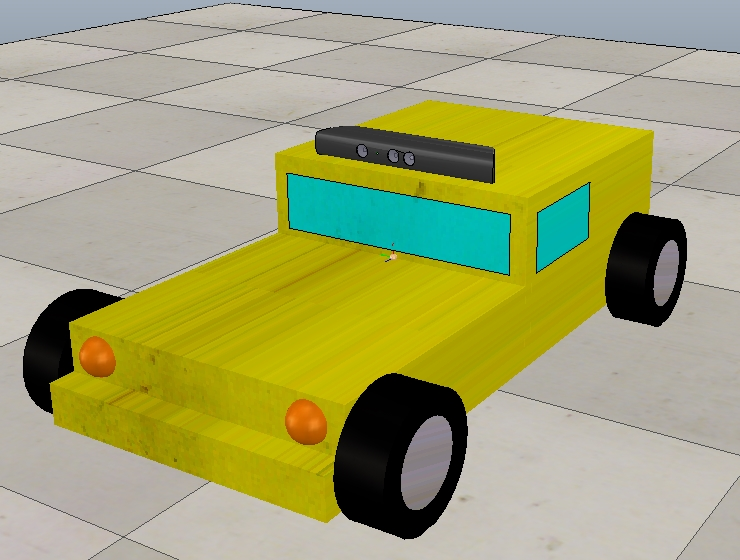
\includegraphics[width=.8\linewidth]{car.jpg}
	\caption{Model samochodu}
	\label{fig:model}
\end{figure}

Samochód biorący udział w symulacji jest z założenia pojazdem autonomicznym, o wysokim stopniu sztucznej inteligencji. Postrzega on swoje środowisko przez posiadane sensory i~na~podstawie danych identyfikuje wszystkie elementy otoczenia. Stworzenie takiego samochodu wymagałoby jednak ogromnych nakładów czasu i pracy, które są dla nas niedostępne z oczywistych względów. Z tego powodu zdecydowaliśmy się zastosować kilka uproszczeń. Obecny w symulacji model faktycznie posiada jedynie dwa rodzaje czujników: 14 czujników odległości oraz kamerę o niskiej rozdzielczości. Czujniki mają formę wskaźników laserowych, widocznych podczas symulacji, co umożliwia weryfikację poprawności ich działania. Są one rozmieszczone naokoło samochodu w rozkładzie: 2 z przodu, 2 z tyłu, po 3 na każdym boku i jeden na każdym rogu pojazdu. Czujniki zwracają odległość samochodu od innych nieprzenikalnych elementów symulacji, co umożliwia określenie czy przed lub za modelem znajduje się inny pojazd. Kamera zamieszczona na dachu pojazdu zwraca obraz RGB o niskiej rozdzielczości. Jeżeli pozwoli na~to~czas realizacji projektu, obraz ten wykorzystany zostanie do wykrywania aktualnego koloru sygnalizacji świetlnej. W przeciwnym wypadku stan świateł przekazywany będzie bezpośrednio do~wiadomości pojazdu. Inne czujniki, umożliwiające takie rzeczy, jak wykrywanie nawierzchni, identyfikację znaków drogowych oraz obserwację ruchu innych modeli znajdujących się w pobliżu, nie zostały fizycznie umieszczone ani zaimplementowane w modelu. Dane te przesyłane będą bezpośrednio z symulacji do poszczególnych pojazdów.

\begin{figure}[!h]
	\centering
	\subfloat[] {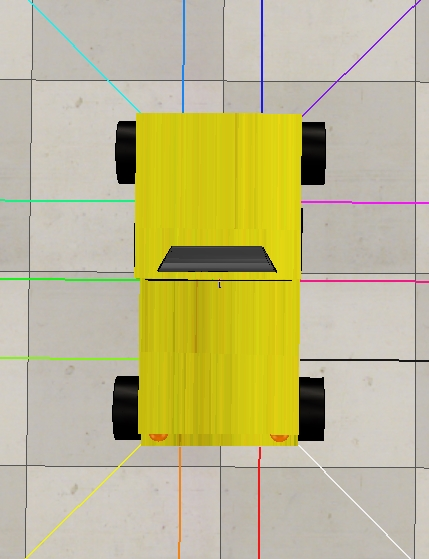
\includegraphics[width=.33\linewidth]{car_sensors.jpg}} \hspace{0.2cm}
	\subfloat[] {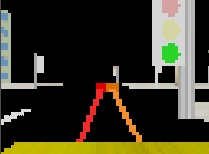
\includegraphics[width=.58\linewidth]{car_kinect.jpg}}
	\caption{Funkcjonalności pojazdu: (a) działanie czujników odległości, (b) obraz widziany z kamery.}
	\label{fig:model_fun}
\end{figure}
